\documentclass{standalone}
\usepackage[utf8]{inputenc}
\usepackage{polski}

\usepackage{listings}
	\lstset{basicstyle=\ttfamily}
	\lstset{escapeinside=\%\%}
	\lstset{tabsize=4}

\usepackage{tikz}
	\usetikzlibrary{matrix}
	\tikzstyle{packet}=[
			shape = rectangle,
			text width = 256pt,
			inner xsep = 8pt,
			inner ysep = 8pt,
		]

\begin{document}
	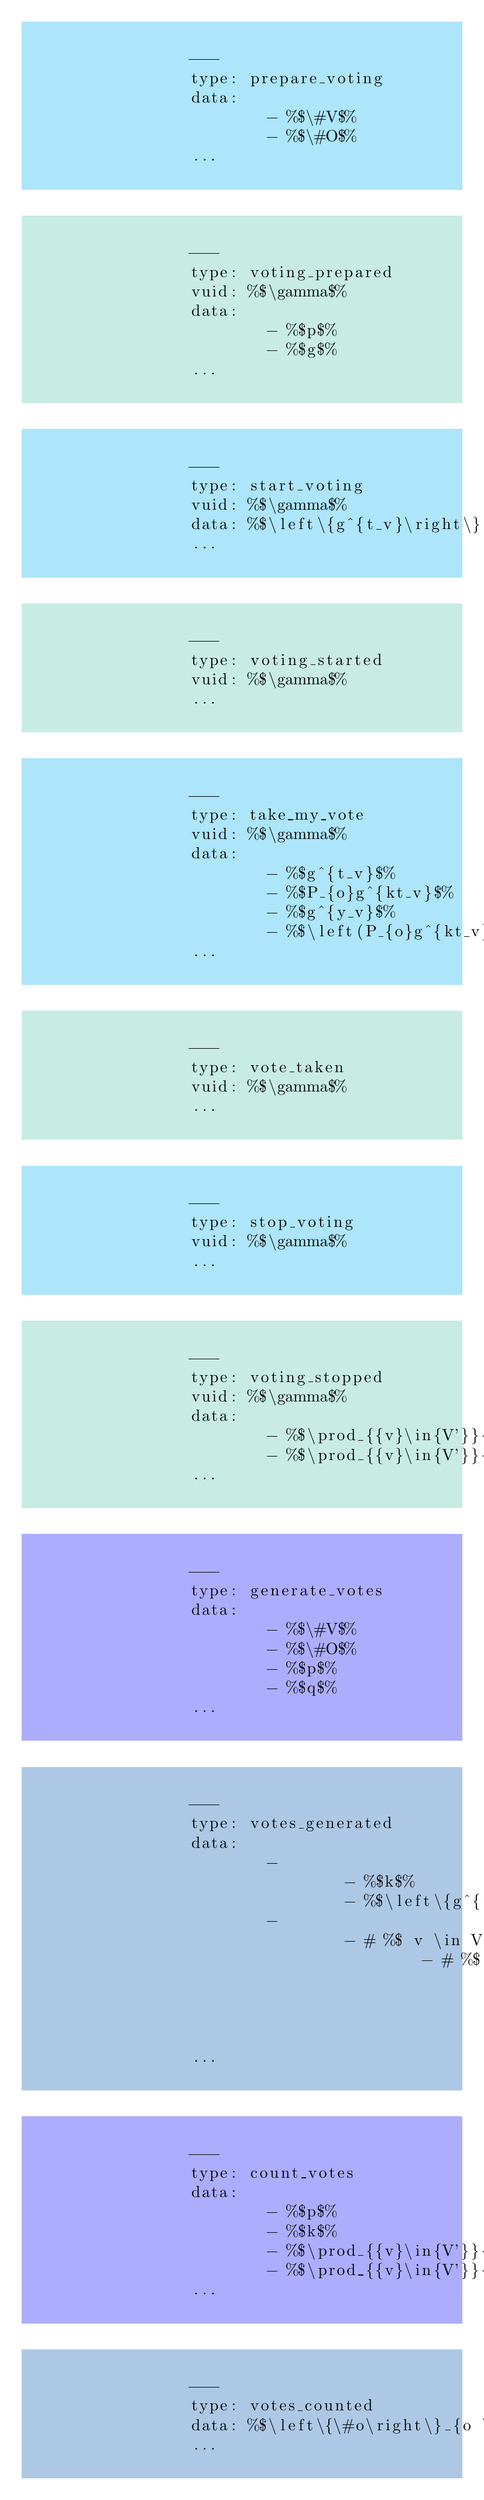
\begin{tikzpicture}

		\matrix [column sep = 64pt, row sep = 16pt]
		{
			\node[packet,fill=cyan!32]{
			\begin{lstlisting}[gobble=16]
				---
				type: prepare_voting
				data:
					- %$\#V$%
					- %$\#O$%
				...
			\end{lstlisting}};
			\\
			\node[packet,fill=yellow!32!cyan!32]{
			\begin{lstlisting}[gobble=16]
				---
				type: voting_prepared
				vuid: %$\gamma$%
				data:
					- %$p$%
					- %$g$%
				...
			\end{lstlisting}};
			\\
			\node[packet,fill=cyan!32]{
			\begin{lstlisting}[gobble=16]
				---
				type: start_voting
				vuid: %$\gamma$%
				data: %$\left\{g^{t_v}\right\}_{v \in V}$%
				...
			\end{lstlisting}};
			\\
			\node[packet,fill=yellow!32!cyan!32]{
			\begin{lstlisting}[gobble=16]
				---
				type: voting_started
				vuid: %$\gamma$%
				...
			\end{lstlisting}};
			\\
			\node[packet,fill=cyan!32]{
			\begin{lstlisting}[gobble=16]
				---
				type: take_my_vote
				vuid: %$\gamma$%
				data:
					- %$g^{t_v}$%
					- %$P_{o}g^{kt_v}$%
					- %$g^{y_v}$%
					- %$\left(P_{o}g^{kt_v}-t_vg^{y_v}\right)y_v^{-1}$%
				...
			\end{lstlisting}};
			\\
			\node[packet,fill=yellow!32!cyan!32]{
			\begin{lstlisting}[gobble=16]
				---
				type: vote_taken
				vuid: %$\gamma$%
				...
			\end{lstlisting}};
			\\
			\node[packet,fill=cyan!32]{
			\begin{lstlisting}[gobble=16]
				---
				type: stop_voting
				vuid: %$\gamma$%
				...
			\end{lstlisting}};
			\\
			\node[packet,fill=yellow!32!cyan!32]{
			\begin{lstlisting}[gobble=16]
				---
				type: voting_stopped
				vuid: %$\gamma$%
				data:
					- %$\prod_{{v}\in{V'}}{g^{t_v}}$%
					- %$\prod_{{v}\in{V'}}{P_{c_v}g^{kt_v}}$%
				...
			\end{lstlisting}};
			\\
			\node[packet,fill=blue!32]{
			\begin{lstlisting}[gobble=16]
				---
				type: generate_votes
				data:
					- %$\#V$%
					- %$\#O$%
					- %$p$%
					- %$q$%
				...
			\end{lstlisting}};
			\\
			\node[packet,fill=green!32!blue!32]{
			\begin{lstlisting}[gobble=16]
				---
				type: votes_generated
				data:
					-
						- %$k$%
						- %$\left\{g^{t_v}\right\}_{v \in V}$%
					-
						- # %$ v \in V $%
							- # %$ o \in O $%
								- %$g^{t_v}$%
								- %$P_{o}g^{kt_v}$%
								- %$g^{y_v}$%
								- %$\left(P_{o}g^{kt_v}-t_vg^{y_v}\right)y_v^{-1}$%
				...
			\end{lstlisting}};
			\\
			\node[packet,fill=blue!32]{
			\begin{lstlisting}[gobble=16]
				---
				type: count_votes
				data:
					- %$p$%
					- %$k$%
					- %$\prod_{{v}\in{V'}}{g^{t_v}}$%
					- %$\prod_{{v}\in{V'}}{P_{c_v}g^{kt_v}}$%
				...
			\end{lstlisting}};
			\\
			\node[packet,fill=green!32!blue!32]{
			\begin{lstlisting}[gobble=16]
				---
				type: votes_counted
				data: %$\left\{\#o\right\}_{o \in O}$%
				...
			\end{lstlisting}};
			\\
		};

	\end{tikzpicture}
\end{document}
